\chapter{Números (4º Bimestre)}

\section{Uso de letras e equação}

We have seen several times in the past that we can use letters to express
formulas. For example the area of side a square of side $3\text{cm}$ is
$3 \times 3 = 9 \text{cm}$. To express the general formula, we say that if
$l$ is the length of one side of a square and $A$ is its area, we have
$A =  l^2$. We also noted that we perform the usual operations on these letters.
We saw that $2^3 \times 2^2 = 8 \times 4 = 32 = 2^{5} = 2^{3+2}$. In general,
this is written $N^p \times N^q = N^{p+q}$ for any natural numbers $N, p, q$.

In an equação, we have a letter $x$ representing an unknown value and an
equality where $x$ is involved, for example $x^2 = 9$. We try to find which
values of $x$ satifisfy the equality and such a value is called a solution
of the equation. $3$ is a solution of the previous equation since $3^2 = 9$
but $2$ is not a solution since $2^2 = 4 \neq 9$. $-3$ is another solution.

\subsection*{Exercício 1}

We consider a circumference together with circumscribed and inscribed polygons.

\begin{center}
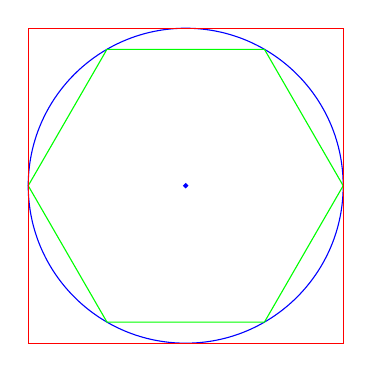
\begin{tikzpicture}
  \begin{scope}[scale=.5]
  \draw (0,0) circle(4)[color=blue];
  \draw[fill=black] (0,0) circle(.05)[color=blue];
  \draw (4,0) -- (2,3.464101615137754) -- (-2,3.464101615137754) --
  (-4,0) -- (-2,-3.464101615137754) -- (2,-3.464101615137754) -- (4,0)
        [color=green];
   \draw[color=red](-4,-4) -- (4,-4) -- (4,4) -- (-4,4) -- cycle;
  \end{scope}
  \end{tikzpicture}
\end{center}

\begin{enumerate}
\item Let $R$ be the radius of the blue circumference and $L$ be its length.
  Recall the expression of $L$ in function of $R$ and $\pi$.
\item What is the length of the side of the red square in function of $R$?
  Express the perimeter $M$ of the red square in function of $R$.
\item Recall the length of a side of the green hexagon.
  Express its perimeter $m$ in function of $R$.
\item Compare $m, L, M$.
\item Deduce the inequality $3 < \pi < 4$.
\end{enumerate}

\subsection*{Exercício 2}

We consider the equation $5x - x^3 = 6 - 2x^2$ where $x$ is an unknown integer.
Verify if the following values are solutions:

\begin{enumerate}
\item $x=0$?
\item $x=1$?
\item $x=-1$?
\item $x=2$?
\item $x=-2$?
\item $x=3$?
\item $x=-3$?
\end{enumerate}

Given a positive integer $a$, can both $a$ and $-a$ be solution of the equation?

\section{Resolução de equações}

Given an equality $A = B$ of two expressions $A,B$ we can add a same expression
$C$ to each side: $A + C = B + C$. We can also substract
a same expression: $A - C = B - C$. Note that by substracting $C$ from the
equality $A + C = B + C$ we come back to the equality $A = B$ so
the $A = B$ and $A + C = B + C$ are equivalent. Similarly, they are
equivalent to $A - C = B - C$.

If $C$ is an expression that does not take a zero value then we can
also multiply and divide an equality $A = B$ by a same value $C$ and
so the equality is equivalent to $\frac{A}{C} = \frac{B}{C}$ and to
$A \times C  = B \times C$. Note that $2 \times 0 = 0 = 3 \times 0$
but $2 \neq 3$, so assuming that $C$ does not take a zero value is important.

If $A = 0$ or $B = 0$ we have $A \times B = 0$. Conversely suppose
that $A \times B = 0$. If $A \neq 0$ then by dividing both sides by $A$
we get $B=0$. Similarly, if $B \neq 0$ then by dividing both sides by $B$
we get $A=0$. So $A=0$ or $B=0$. Say otherwise we have the equivalence:
a product is null if and only if one of its factor is null.

We can combine all these techniques to solve equation. For instance,
consider the equation
%%
$$\frac{6}{y} -3 = y - 2$$
%%
for some unknown number $y \neq 0$. This is equivalent to the equation
obtained by multiplying both sides by $y$:

$$6 - 3y = \left(y - 2\right) \times y$$

This is equivalent to the equation obtained by adding
$\left(y - 2\right) \times 3 = 3y - 6$ to both sides:

$$6 - 3y + 3y - 6 = \left(y - 2\right) \times y + 
\left(y - 2\right) \times 3$$

which can be simplified as
$$0 = \left(y - 2\right)\left(y + 3\right)$$

Now the product is null if and only if $y - 2 = 0$ or $y + 3 = 0$. This is
equivalent to $y = 2$ or $y = -3$. By the equivalence, these are
exactly the only solutions of the equation. We can verify that
$\frac{6}{2} - 3 = 0 = 2 - 2$ and $\frac{6}{-3} - 3 = -5 = -3 - 2$.

As another example, consider an unknown $z$ that satisfies both
$z^2 + z = 1$ and $-z^2 + z = 3$. We can sum up each side of the equation to
obtain $z^2 + z - z^2 + z = 1 + 3$ that is $2z = 4$ and finally $z = 2$.
However, $2^2 + 2 = 6 \neq 1$ and $-2^2 + 2 = -2 \neq 3$. So the sum of the
initial equation is not equivalent to the conjunction of the individual
equation. This also shows that this conjunction does not have any solution.

\subsection*{Exercício 3}

Solve the following equations with unknown $x$:

\begin{enumerate}
\item $3x + 7 = 2x - 5$
\item $x^2 + 5 = 3x^2 + 7$
\item $x^2 + 5 = 3x^2 - 3$
\item $\frac{1}{x} = \frac{x}{16}$ for $x \neq 0$.
\item $\left(x - 7\right)\left(x + 5\right) = 0$
\end{enumerate}

\subsection*{Exercício 4}

We consider a real number $u$ such that $u^2=3$. Let
$P = x^2 + \left(\frac{5}{2} - u\right)x - \frac{5u}{2}$. We want to solve the
equation $P = 0$ with unknown $x$.

\begin{enumerate}
\item Is $x=0$ a solution?
\item Let $Q = \left(x + \frac{5}{4} - \frac{u}{2}\right)^2$. Show that
  $Q - P = \frac{20u+37}{16}$
\item Find integers $a,b$ such that
  $\left(\frac{au+b}{4}\right)^2 = Q - P$.
\item Express the solutions of the equation $P=0$ in function of $u$.
\item Verify that indeed
  $x^2 + \left(\frac{5}{2} - u\right)x - \frac{5u}{2} = 0$ for the
  solutions found.
\end{enumerate}

\subsection*{Exercício 5 (problem)}

Note: we admit that the area of a disc of radius $R$ is given by the formula
$A_R = \pi R^2$.
We cut a rope of length $L$ into two parts: a rope of length $0 \leq x \leq L$
from which we make a square and a rope of length $L - x$ from which we make
a circumference.

\begin{enumerate}
\item Express the side of the square and the radius of the circumference in
  function of $x$.
\item Express the areas of the square and disc in function of $x$.
\item We find constants $a,b$ such that the sum of areas
  of the square and disc is written
%%
  $$
  A(x) = a \left( x - \frac{4L}{\pi+4}\right)^2 + b
  $$

  Show that $a \frac{16L^2}{\left(\pi+4\right)^2} + b = \frac{L^2}{4\pi}$ (1)
  and $a \frac{\pi^2L^2}{\left(\pi+4\right)^2} + b = \frac{L^2}{16}$ (2)

\item Expand ${(4-\pi)}{(4+\pi)}$. By subtracting (1) and (2) deduce that
  $a = \frac{\pi+4}{16\pi}$.

\item Show that $b = \frac{L^2}{4\left(\pi+4\right)}$

\item Verify that the expression $A(x)$ with the values $a,b$ found is indeed
  the sum of the two areas.
  
\item Find $0 \leq x_0 \leq L$ such that $A(x_0) = b$.

\item Compare $A(x), A(x_0)$ when $x \neq x_0$. What can you say about $x_0$?
\end{enumerate}

\section{Solução dos exercícios}

\subsection*{Exercício 1}

\begin{enumerate}
\item $L = 2 \times \pi \times R$
\item This is a square of side $2R$ so its perimeter is
  $M = 4 \times 2R = 8R$.
\item The side of the hexagon is $R$ so its perimeter is
  $m = 6R$.
\item As we can see on the figure, $m < L < M$.
\item The previous expressions become $6R < 2 \times \pi \times R < 8R$.
  If we divide everything by $2R$ we find
  $3 = \frac{6R}{2R} < \pi < \frac{8R}{2R} = 4$.  
\end{enumerate}

\subsection*{Exercício 2}

\begin{enumerate}
\item $5x - x^3 = 0 \neq 6 = 6 - 2x^2$ so $0$ is not a solution.
\item $5x - x^3 = 4 = 6 - 2x^2$ so $1$ is a solution.
\item $5x - x^3 = -4 \neq 4 = 6 - 2x^2$ so $1$ is not a solution.
\item $5x - x^3 = 2 \neq -2 = 6 - 2x^2$ so $2$ is not a solution.
\item $5x - x^3 = -2 = -2 = 6 - 2x^2$ so $-2$ is a solution.
\item $5x - x^3 = -12 = -12 = 6 - 2x^2$ so $3$ is a solution.
\item $5x - x^3 = 12 \neq -12 = 6 - 2x^2$ so $-3$ is not a solution.
\end{enumerate}

We already verified that we can not have both $a$ and $-a$ solutions for
$a = 0,1,2,3$. If $x=a$ is a solution then $5a - a^3 = 6 - 2a^2$.
If $x=-a$ is also a solution then $-5a + a^3 = 6 - 2a^2$.
Hence $5a - a^3 = -5a + a^3$. We can divide everything by $a \neq 0$ and we
get $5 - a^2 = -5 + a^2$ that is $2a^2 = 10$ and finally $a^2 = 5$. But
if $a \geq 4$ we have $a^2 \geq 16 > 5$ so the previous equality never happens.

\subsection*{Exercício 3}

\begin{enumerate}
\item $3x + 7 = 2x - 5$. By adding $-2x-7$ to both sides, this is equivalent
  to $x = -12$.
\item $x^2 + 5 = 3x^2 + 7$. By adding $-x^2 - 7$ to both sides, 
  this is equivalent to $-2 = 2x^2$. But for any real number $r$, we
  have $2r^2 \geq 0$ so the equation does not have any solution.
\item $x^2 + 5 = 3x^2 - 3$. By adding $-x^2 + 3$ to both sides,
  this is equivalent to $8 = 2x^2$ that is $x^2 = 4$. There are exactly
  two solutions: $x = 2$ and $x = -2$.
\item $\frac{1}{x} = \frac{x}{16}$. By multiplying by $16x \neq 0$ this is
  equivalent to $16 = x^2$. There are exactly two solutions:
  $x = 4$ and $x=-4$.
\item $\left(x - 7\right)\left(x + 5\right) = 0$ if and only if
  $x - 7 = 0$ or $x+5=0$. There are  exactly two solutions:
  $x = 7$ and $x=-5$.
\end{enumerate}

\subsection*{Exercício 4}

\begin{enumerate}
\item For $x=0$ we get $P = -\frac{5u}{2}$. If $x=0$ is a solution then
  $P=-\frac{5u}{2}=0$ that is $u=0$. But this contradicts $u^2 = 3$ so
  $x=0$ is not a solution.
\item
  $Q = x^2 + \frac{25}{16}+\frac{u^2}{4} - \frac{5}{2}x - ux - \frac{5u}{4}$
  so $Q - P = \frac{5u}{4} + \frac{5u}{2} + \frac{25}{16} + \frac{3}{4} =
  \frac{20u+37}{16}$.
\item We have $\left(\frac{au+b}{4}\right)^2 = \frac{a^2u^2+b^2+2abu}{16} =
  \frac{2abu + 3a^2+b^2}{16}$. So it is enough to
  have $ab = 10$ and $3a^2+b^2=37$. We try to factorize $10$ as a product
  of two integers $a,b$. For $a=1,b=10$ we have $3a^2+b^2=103 \neq 37$.
  For $a=2,b=5$ we have $3a^2+b^2 = 37$ so this is one possibility.
\item If $P=0$ we get
  $\left(\frac{2u+5}{4}\right)^2 = Q =
  \left(x + \frac{5}{4} - \frac{u}{2}\right)^2 =
  \left(\frac{4x+5-2u}{4}\right)^2$. This is equivalent to
  $2u+5 = 4x+5-2u$ or $-2u-5 = 4x+5-2u$.
  Finally we find two solutions: $x = u$ or $x = -\frac{5}{2}$.
\item For $x=u$ we find
  $P=u^2 + \left(\frac{5}{2} - u\right)u - \frac{5u}{2} =
  u^2 - u^2 + \frac{5}{2}u - \frac{5u}{2} = 0$. For $x = -\frac{5}{2}$
  we find
  $P = \left(-\frac{5}{2}\right)^2 + \left(\frac{5}{2} - u\right) -\frac{5}{2}
  - \frac{5u}{2} =
  \frac{25}{4}  -\frac{25}{4} + \frac{5}{2}u - \frac{5u}{2} = 0$.
\end{enumerate}

\subsection*{Exercício 5 (problem)}

\begin{enumerate}
\item Los perimetros son $4c = x$ y $2 \pi r = L - x$ entonces
  el lado del cuadro es $c = \frac{x}{4}$ y el radio del círculo es
  $r = \frac{L-x}{2 \pi}$.
\item La area del cuadro es $c^2 = \frac{x^2}{16}$ y la area del disco
  es $\pi r^2 = \frac{{(L-x)}^2}{4\pi}$.

\item When $x= L$, the total area is the one of the square of side
  $\frac{L}{4}$. When $x = 0$, the total area is the one of the disc of
  radius $\frac{L}{2\pi}$.
  Hence $A(0) = \frac{L^2}{4\pi}$ and $A(L) = \frac{L^2}{16}$. If we want
  to find $a,b$ such that
%%
  $$
  A(x) = a \left( x - \frac{4L}{\pi+4}\right)^2 + b
  $$

  then this becomes
  $A(0) = a \frac{16L^2}{\left(\pi+4\right)^2} + b = \frac{L^2}{4\pi}$
  and $A(L) = 
  a \left(\frac{\pi+4-4}{\pi+4}L\right)^2 + b =
  a \frac{\pi^2L^2}{\left(\pi+4\right)^2} + b = \frac{L^2}{16}$.

\item We note that ${(4-\pi)}{(4+\pi)} = 16 - \pi^2$.
  So subtracting (1) and (2) gives
  $a \frac{{(4-\pi)}{(4+\pi)}}{\left(\pi+4\right)^2} L^2 =
  \frac{L^2}{4\pi} - \frac{L^2}{16}$, that is
%%
  $$a \frac{4-\pi}{\pi+4} L^2 = \frac{4-\pi}{16\pi} L^2$$

  Dividing both sides by ${(4-\pi)} L^2 \neq 0$ we get
  $\frac{a}{\pi+4} = \frac{1}{16\pi}$ and finally
  $a = \frac{\pi+4}{16\pi}$
  
\item Reinjecting $a$ in either (1) or (2), we can solve a simple
  equation to find $b = \frac{L^2}{4\left(\pi+4\right)}$.

\item The sum of the areas is
  $\frac{x^2}{16} + \frac{\left(L-x\right)^2}{4\pi} =
  \frac{\pi}{16\pi}x^2 + \frac{L^2 - 2xL + x^2}{4\pi} =
  \frac{\pi+4}{16\pi} x^2 - \frac{L}{2\pi}x + \frac{L^2}{4\pi}$.
  Our assumed formula is
  $A(x) = a \left( x - \frac{4L}{\pi+4}\right)^2 + b =
  \frac{\pi+4}{16\pi} x^2 - \frac{\pi+4}{16\pi} \frac{8L}{\pi+4} x +
  \frac{\pi+4}{16\pi} \frac{16L^2}{\left(\pi+4\right)^2} +
  \frac{L^2}{4\left(\pi+4\right)}$. After simplification, we notice that
  indeed the two expressions are the same.

\item $A(x_0) = b$ becomes $a \left(x_0 - \frac{4L}{\pi+4}\right)^2 = 0$,
  which is equivalent to $x_0 - \frac{4L}{\pi+4} = 0$, that is
  $x_0 = \frac{4L}{\pi+4}$.
  We note that $0 \leq \frac{4L}{\pi+4} \leq \frac{4L}{0+4} = L$.
  
\item If $x \neq x_0$ then it is not solution to
  $A(x_0) = b$ and so $a \left(x_0 - \frac{4L}{\pi+4}\right)^2 \neq 0$.
  Actually, since $a > 0$ and a square is always nonnegative we have
  $a \left(x_0 - \frac{4L}{\pi+4}\right)^2 > 0$
  so $A(x) > A(x_0)$. Hence cutting the rope at $x_0$ provides the minimal sum
  of areas for the disc and square.
\end{enumerate}

